\documentclass{article}

\usepackage{fullpage}
\usepackage{color}
\usepackage{amsmath}
\usepackage{url}
\usepackage{verbatim}
\usepackage{graphicx}
\usepackage{parskip}
\usepackage{amssymb}
\usepackage{nicefrac}
\usepackage{listings} % For displaying code
\usepackage{algorithm2e} % pseudo-code

\def\rubric#1{\gre{Rubric: \{#1\}}}{}
    
% Colors
\definecolor{blu}{rgb}{0,0,1}
\def\blu#1{{\color{blu}#1}}
\definecolor{gre}{rgb}{0,.5,0}
\def\gre#1{{\color{gre}#1}}
\definecolor{red}{rgb}{1,0,0}
\def\red#1{{\color{red}#1}}
\def\norm#1{\|#1\|}
    
% Math
\def\R{\mathbb{R}}
\def\argmax{\mathop{\rm arg\,max}}
\def\argmin{\mathop{\rm arg\,min}}
\newcommand{\mat}[1]{\begin{bmatrix}#1\end{bmatrix}}
\newcommand{\alignStar}[1]{\begin{align*}#1\end{align*}}
\def\half{\frac 1 2}
    
% LaTeX
\newcommand{\fig}[2]{\includegraphics[width=#1\textwidth]{#2}}
\newcommand{\centerfig}[2]{\begin{center}\includegraphics[width=#1\textwidth]{#2}\end{center}}
\newcommand{\matCode}[1]{\lstinputlisting[language=Matlab]{a2f/#1.m}}
\def\items#1{\begin{itemize}#1\end{itemize}}
\def\enum#1{\begin{enumerate}#1\end{enumerate}}
    
\begin{document}
    
\title{CPSC 340 Assignment 3 (due Friday, Oct 12 at 11:55pm)}
\date{}
\maketitle
    
\vspace{-7em}

\section{Finding Similar Items}
\subsection{Exploratory data analysis}

\subsubsection{Most popular item}
Item: Classic Accessories 73942 Veranda Grill Cover - Durable BBQ Cover with Heavy-Duty Weather Resistant Fabric, X-Large, 70-Inch
Number of Stars: 14454

\subsubsection{User with most reviews}
User ID: A100WO06OQR8BQ, Number of Items: 161

\subsubsection{Histograms}
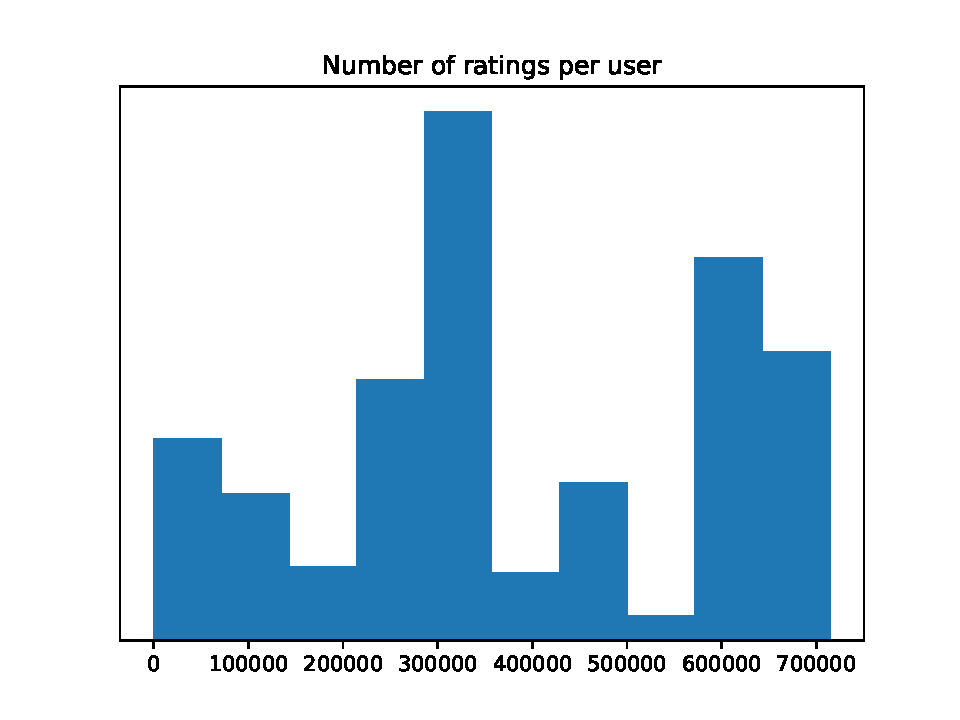
\includegraphics[scale=0.5]{q111.pdf}
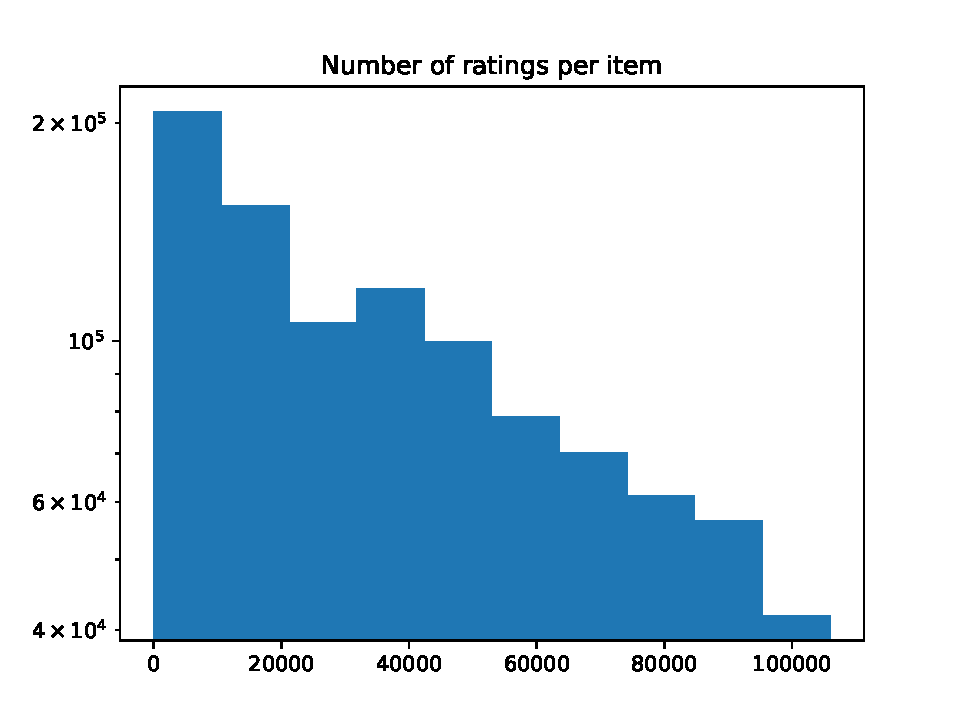
\includegraphics[scale=0.5]{q112.pdf}\\

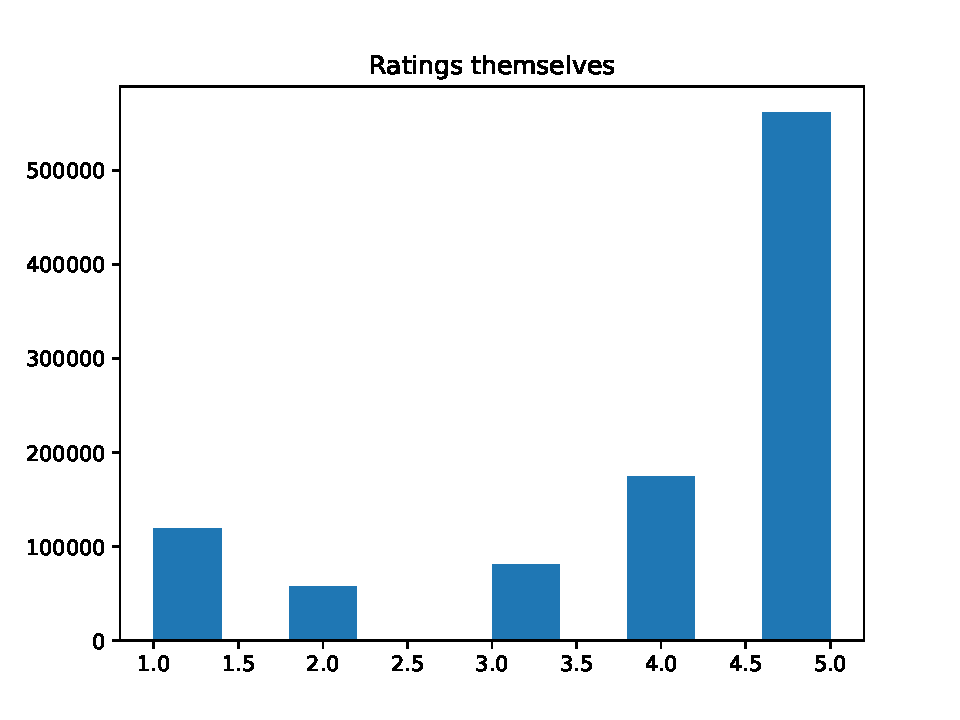
\includegraphics[scale=0.5]{q113.pdf}

\section{Matrix Notation and Minimizing Quadratics}
\subsection{Converting to Matrix/Vector/Norm Notation}
\begin{enumerate}
    \item $||Xw - y||_{\infty}$
    \item $(Xw-y)^TV(Xw-y)+\frac{\lambda}{2}||w||_2$
    \item $|Xw-y|^2_1+\frac{1}{2}A|w|_1$
\end{enumerate}

\subsection{Minimizing Quadratic Functions as Linear Systems}
\begin{enumerate}
    \item 
    \begin{equation*}
        \begin{split}
        \frac{1}{2}||w-v||^2 &= \frac{1}{2}(w^T-v^T)(w-v)\\
        &= \frac{1}{2}w^Tw-w^Tv-\frac{1}{2}v^Tv\\
        &= w - v \\
        w - v &= 0 \\
        w &= v\\
        \end{split}
    \end{equation*}
    \item 
    \begin{equation*}
        \begin{split}
        \frac{1}{2}||Xw-y||^2+\frac{1}{2}w^TAw &= \frac{1}{2}(w^TX^T-y)(Xw-y)+\frac{1}{2}w^TAw \\
        &= \frac{1}{2}w^TX^TXw - w^TX^Ty - \frac{1}{2}y^Ty + \frac{1}{2}w^TAw\\
        &= X^TXw - X^Ty + Aw\\
        X^TXw - X^Ty + Aw &= 0\\
        w(X^TX + AI) &= + X^Ty\\
        \end{split}
    \end{equation*}
    \item 
    \begin{equation*}
        \begin{split}
        \frac{1}{2}\sum_{i=1}^{n}v_i(w^Tx_i-y_i)^2+\frac{\lambda}{2}||w-w^0||^2 &= v\frac{1}{2}(w^TX^T-y)(Xw-y)+\frac{\lambda}{2}(w^T-(w^0)^T)(w-w^0)\\
        &= v(\frac{1}{2}w^TX^TXw - w^TX^Ty - \frac{1}{2}y^Ty)+\frac{\lambda}{2}w^Tw-\lambda w^Tw^0+\frac{\lambda}{2}(w^0)^Tw^0)\\
        &= vX^TXw-vX^Ty-\lambda w-\lambda w^0\\
        vX^TXw-vX^Ty-\lambda w-\lambda w^0 &= 0\\
        vX^TXw -\lambda w &= vX^Ty + \lambda w^0\\
        w(X^TXw -\lambda I) &= vX^Ty + \lambda w^0\\
        \end{split}
    \end{equation*}
\end{enumerate}

\section{Robust Regression and Gradient Descent}
\subsection{Weighted Least Squares in One Dimension}
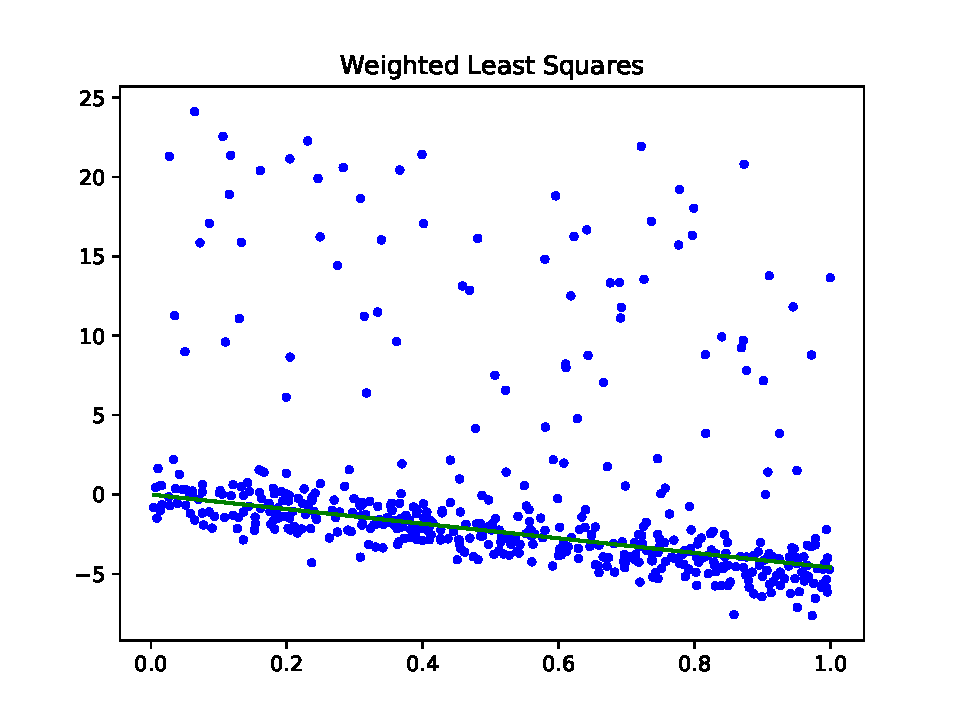
\includegraphics[scale = 0.5]{31WLS.pdf}

\subsection{Smooth Approximation to the L1-Norm}
\begin{equation*}
    \begin{split}
    \nabla F &= \frac{d}{dr}[log(exp(r)+exp(-r))]\\
    &= \frac{exp(r)-exp(-r)}{exp(r)+exp(-r)}\\
    \frac{\partial f}{\partial w_j} &= \sum_{i=1}^n  x_{ij} \frac{exp(w^Tx_i-y_i)-exp(y_i-w^Tx_i)}{exp(w^Tx_i-y_i)+exp(y_i-w^Tx_i)}\\
    r_i &= \frac{exp(w^Tx_i-y_i)-exp(y_i-w^Tx_i)}{exp(w^Tx_i-y_i)+exp(y_i-w^Tx_i)}\\
    &= X^T\frac{exp(Xw-y)-exp(y-Xw)}{exp(Xw-y)+exp(y-Xw)}\\
    \end{split}
\end{equation*}
\subsection{Robust Regression}
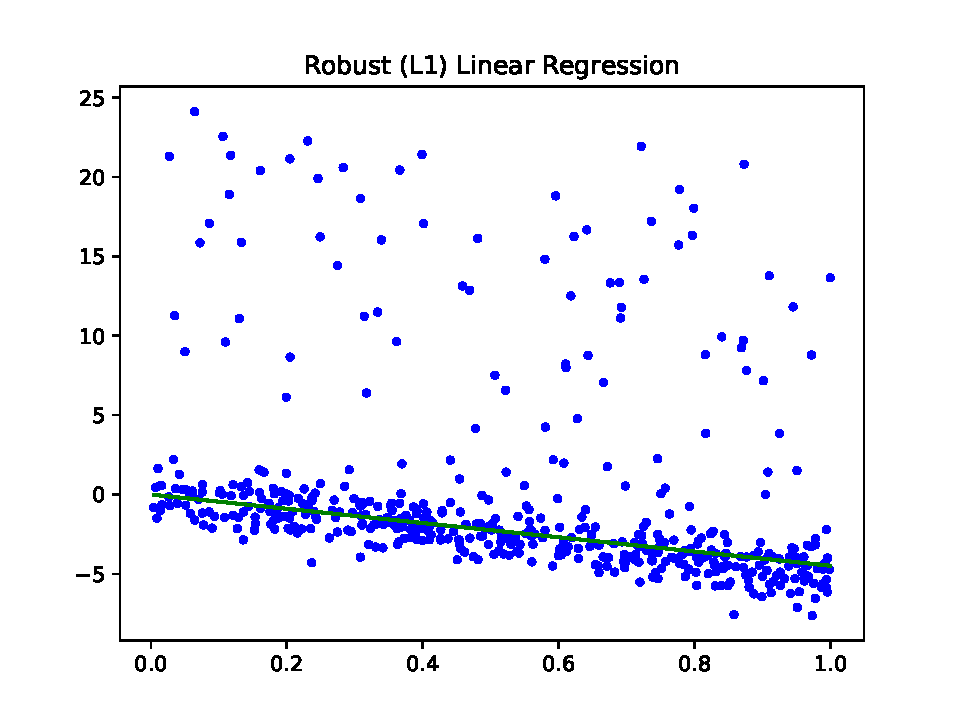
\includegraphics[scale = 0.5]{least_squares_robust.pdf}

\section{Linear Regression and Nonlinear Bases}
\subsection{Adding a Bias Variable}
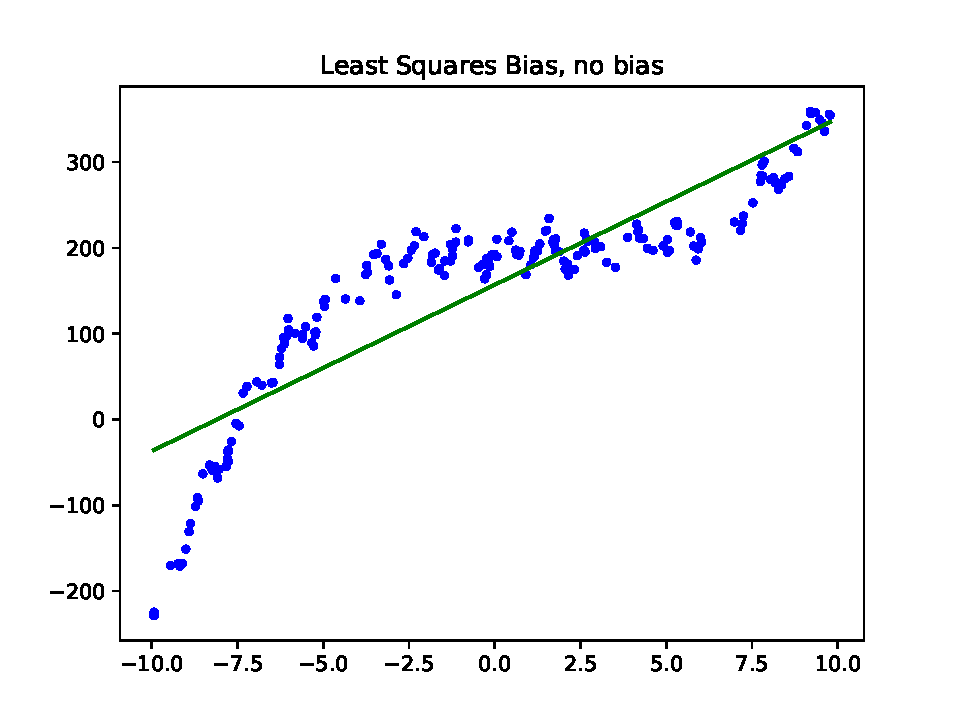
\includegraphics[scale=0.5]{41LSB.pdf}

\subsection{Polynomial Basis}
p=0
Training error = 15480.5
Test error     = 14390.8\\
p=1
Training error = 3551.3
Test error     = 3393.9\\
p=2
Training error = 2168.0
Test error     = 2480.7\\
p=3
Training error = 252.0
Test error     = 242.8\\
p=4
Training error = 251.5
Test error     = 242.1\\
p=5
Training error = 251.1
Test error     = 239.5\\
p=6
Training error = 248.6
Test error     = 246.0\\
p=7
Training error = 247.0
Test error     = 242.9\\
p=8
Training error = 241.3
Test error     = 246.0\\
p=9
Training error = 235.8
Test error     = 259.3\\
p=10
Training error = 235.1
Test error     = 256.3\\
Generally, as the degree of the polynomial increased, the training error and test error decreased and the amount
it decreases becomes less and less as p gets larger.
\section{Very-Short Answer Question}
\begin{enumerate}
    \item For a global outlier in K-Means, the outlier will be assigned the nearest mean value and the mean value 
    will be not as close to the other points to accommadate for the global outlier. In clustering, the global outlier 
    will not be assigned to anything as the outlier only consists of itself and there would be no clustering whatsoever.
    \item Random restarts are necessary for k-means because the the means in k-means will be initialized randomly. Increasing
    the number of restarts will decrease the effects of random initialization. It is unnecessary for density clustering
    because density clustering looks at the points around a radius of given points rather than randomly initialized means.
    \item Yes
    \item Computing the z score. A problem is that this model assumes that the data is centered around the mean which may not be true.
    \item Boxplots. A problem with boxplots is that it looks at only 1 variable at a time
    \item Decision Trees. A problem is that we need to label a data set to be of non-outliers and outliers and we may not detect
    other outliers since it may train on limitied data that does not have all types of outliers.
    \item Gradient descent would not be needed as it is easy to use the ordinary linear squares solution since d is small (d=1). Computing
    the ordinary least squares would only require $O(n)$ time where as $O(nt)$ for gradient descent
    \item We only add the column of 1 values to X because we need to accommadate for the y-intercept $\beta$. It would not make
    sense to add this column to the training set for decision trees. 
    \item If a function is convex, it will have at most 1 stationary/critical point. The critical/stationary point may not exist
    such as in the case of absolute value function. There will always be a minimizer and a minimum point for convex functions.
    \item If the learning rate is too small, we may need many iterations to converge to the best values.
    \item If the learning rate is too big, we may skip over the optimal solution.
    \item If we were to look for the gradient of an absolute function, it may not exist. The purpose of log-sum-exp is to Smooth
    out the function so we can compute the gradient for the function.
    \item Using a polynomial basis
\end{enumerate}

\end{document}